%%%%%%%%%%%%%%%%%%%%%%% file template.tex %%%%%%%%%%%%%%%%%%%%%%%%%
%
% This is a template file for the LaTeX package SVJour2 for the
% Springer journal "Theoretical Chemistry Accounts"
%
%                                    Springer Heidelberg 2004/12/03
%
% Copy it to a new file with a new name and use it as the basis
% for your article. Delete % as needed.
%
%%%%%%%%%%%%%%%%%%%%%%%%%%%%%%%%%%%%%%%%%%%%%%%%%%%%%%%%%%%%%%%%%%%
%
% First comes an example EPS file -- just ignore it and
% proceed on the \documentclass line
% your LaTeX will extract the file if required
%\begin{filecontents*}{example.eps}
%!PS-Adobe-3.0 EPSF-3.0
%%BoundingBox: 19 19 221 221
%%CreationDate: Mon Sep 29 1997
%%Creator: programmed by hand (JK)
%%EndComments
%gsave
%newpath
%  20 20 moveto
%  20 220 lineto
%  220 220 lineto
%  220 20 lineto
%closepath
%2 setlinewidth
%gsave
%  .4 setgray fill
%grestore
%stroke
%grestore
%\end{filecontents*}
%
\documentclass[twocolumn,fleqn]{svjour2}
%
\smartqed  % flush right qed marks, e.g. at end of proof
%
\usepackage[numbers,sort&compress]{natbib}
%\usepackage{subcaption}
\usepackage{natbib}
\usepackage{graphicx}
\usepackage{adjustbox}
\usepackage{color}
\pagenumbering{arabic}
%
% \usepackage{mathptmx}      % use Times fonts if available on your TeX system
%
% insert here the call for the packages your document requires
%\usepackage{latexsym}
% etc.
%
% please place your own definitions here and don't use \def but
% \newcommand{}{}
%
\newcommand*\mycommand[1]{\texttt{\emph{#1}}}
\journalname{Theoretical Chemistry Accounts}
%
\begin{document} \sloppy

\title{Ability of Density Functional Theory Methods to Accurately Model the Reaction Energy Pathways of the Oxidation of CO on Gold Cluster: A Benchmark Study }

%\subtitle{Do you have a subtitle?\\ If so, write it here}

%\titlerunning{Short form of title}        % if too long for running head

\author{Saumya Gurtu$^{\dagger}$ \and Sandhya Rai$^{\dagger}$ \and Masahiro Ehara$^{\ddagger}$ \and U. Deva Priyakumar$^{\ast,\dagger}$ %etc.
}

%\authorrunning{Short form of author list} % if too long for running head

\institute{ U. Deva Priyakumar \\
           \email{deva@iiit.ac.in}\\
           $^\ast$ To whom correspondence should be addressed. \\ \\
              $^\dagger$ Center for Computational Natural Sciences and Bioinformatics, International Institute of Information Technology, Hyderabad, India.\\ \\
           $^\ddagger$ Research Center for Computational Science, Institute for Molecular Science,
38 Nishigo-Naka, Myodaiji, Okazaki 444-8585, Japan.
}

\date{Received: date / Accepted: date}
% The correct dates will be entered by the editor

\maketitle

\begin{abstract}
Gold clusters are currently regarded as new generation catalysts owing to their exceptional efficiency in accelerating several classes of reactions. Density functional theory (DFT) is the method of choice for the investigation of energy pathways of reactions assisted by metal nanoparticles due to their computational efficiency. However, the reliability of such theoretical studies depends to a large extent on the choice of the DFT functional used. In the present work, the performance of a series of DFT based functionals to accurately model the prototypical CO oxidation reaction catalyzed by a Au$_3$ cluster has been examined by comparing the results with those obtained from high level \textit{ab initio} CCSD(T) method. This comparison study has been carried along the two possible pathways (Eley--Rideal (ER) and the Langmuir--Hinshelwood (LH)). No significant differences among the DFT functionals were observed in terms of obtaining the geometries of stationary points including the transition states with minor exceptions. However, the adsorption energies, barrier heights and reaction energies calculated using the DFT methods lie in a wide range with some methods showing high deviations from the CCSD(T) results. Our calculations suggest that the adsorption energy values are sensitive to the inclusion of long range correction and dispersion correction, whereas the barrier heights do not show much dependence on the inclusion of dispersion effects. The percentage of Hartree-Fock exchange included in the DFT functional also plays a crucial role in predicting the correct pathway. Based on this extensive benchmark study, it is suggested that the computationally less expensive hybrid density functionals, PBE0, B3PW91 and B3P86, are better suited for accurate modeling of this class of reactions.
\keywords{ CO oxidation \and Gold nano cluster \and Heterogeneous catalysis \and Reaction kinetics \and Reaction mechanism }
\end{abstract}

\section{Introduction}
Owing to their extraordinary catalytic potential gold nanoparticles and clusters find significant applications in the field of heterogeneous catalysis \cite{haruta1987,Olga2010}. The chemical oxidation and reduction reactions of small molecules like CO, NO, NO$_2$ etc., catalyzed by gold clusters in the nanometer length scale have gained considerable interest in industrial and academic research because of its remarkable potential in providing a green route to these industrially important reactions \cite{stratakis2012catalysis}. Potential application of nanogold in catalyzing the oxidation process of CO was discovered by Haruta \textit{et. al.} \cite{haruta1987,hashmi2006}. This oxidative process at ambient temperatures, has enormous environmental and commercial importance as it provides a feasible route to the water-gas shift reaction by causing selective oxidation of CO yielding pure H$_2$ \cite{stratakis2012catalysis,okumura2004vital,weiher2007activation}.
It has been observed that Au particles with sizes between 1--6 nm display remarkable catalytic activity for CO oxidation in contrast to bulk metallic gold \cite{Haruta1997,Valden1998,meerson2005}. Apart from the CO oxidation, Au nanoparticles also prove to be powerful catalysts for the oxidation of hydrocarbons, alcohols, amines etc. \cite{della2008selective,della2012update}. These particles also catalyze the synthesis of H$_2$O$_2$ directly from H$_2$ and O$_2$ \cite{hutchings2008nanocrystalline,edwards2013effect,edwards2009switching}.\\
The catalytic properties of the nanoparticles are largely determined by their size, shape and electronic structure, making theoretical studies crucial for understanding the mechanistic pathways of the reactions. Owing to the large system size of metal clusters, the performance and reliability of the theoretical methodologies are important issues that need to be assessed before they are applied to answer relevant questions related to reaction pathways. Application of density functional theory (DFT) based methods have been reported to be more efficient compared to wave function theory (WFT) methods for thermochemistry and kinetics calculations which is attributed to their excellent cost-to-performance ratio \cite{zhao2005}. Additionally, DFT methods can be used to model larger systems involving transition metals that are otherwise difficult or impossible using WFT methods, making  DFT a preferred choice for calculations involving transition elements \cite{ricca1995comparison,siegbahn2006modeling,zhao2008density,cramer2009density}.\\ 
Although DFT methods are practically very efficient in modeling large systems, especially involving metal nanoparticles, choice of the DFT functional is crucial for obtaining quantitative estimations. The performance of DFT methods has to be properly examined before it can be used to obtain chemical insights into a given problem. For example, pure DFT methods are known to overestimate bond energies and underestimate barrier heights in general \cite{zhao2005}, and are further corrected by using hybrid DFT methods which is theoretically justified by the adiabatic connection theorem \cite{becke1993,kohn1996}. Nonetheless, majority of these hybrid DFT functionals are designed for stable systems lying on the minima of a potential energy surface (PES) \cite{Pu2005}. Recently some ``accurate for dynamics" PES methods have been developed, making it feasible to perform reliable calculations of reaction rate constants for larger and complex systems \cite{lynch2000,lynch2003,zhao2004jpca}. \\ 
Though, several GGA functionals have proved useful in applications to transition metals and systems involving non covalent interactions \cite{goerigk2010efficient,goerigk2011thorough}, Perdew, Burke, and Ernzerhof (PBE) have developed a simplified GGA functional that best fulfills many of the physical and mathematical requirements of DFT \cite{perdew1996}. In a recent study, $\omega$B97x-D has been reported to accurately predict the  gas phase enthalpies of formation for 30 second row transition metal-containing molecules.\cite{laury2013} Another study on reaction mechanism involving Pd based catalyst applies B2PLYP-D functional for the prediction of the reaction enthalpies and activation barriers \cite{theil2014}. A very recent study on water gas shift reaction on Ru--EDTA complex has been done using the $\omega$B97x-D method \cite{chen2015}. \\
As discussed above, there have been many computational studies that used DFT methods to investigate reactions involving metal nanoparticles. However, given the intricacies involved in the modeling of such reactions, a systematic study that assesses the performance of various DFT functionals compared to robust \textit{ab initio} methods that often offer a reliable description of chemical reaction pathways is desirable. Enduring interest in studying carbon monoxide, CO, oxidation is attributed to the fact that it is a crucial step in various large scale industrial and medical applications \cite{xie_2009,freund2011}. In addition to that, from the academic view point, this process serves as an archetype to discern the pervasive domain of heterogeneous catalysis \cite{freund2011}. The currently available catalysts for this process are reported to get deactivated rapidly, making them inadequate for long term use \cite{xie_2009}. Hence, development of new viable methods for oxidation of CO is currently considered as one of the key areas in the field of heterogeneous catalysis. This reaction also captures many important features of a typical inorganic reaction, and thus serves as a prototype to understand complex inorganic processes, making it an apt choice to perform the benchmark studies. Two mechanisms have been proposed in literature, via which the oxidative process can proceed \cite{zhang2007,lopez2002,mavrikakis2003,liu2002,liu2003}; (1) ER mechanism, where O$_2$ molecules react with CO molecules that are preadsorbed on the catalyst surface, (2) LH mechanism, where coadsorption of the two reactants (CO and O$_2$) on the catalyst is the first step of the reaction (see later). It has been reported that LH mechanism is more favorable in context of the oxidation process \cite{zhang2007,Gruene2008,Olga2010,Jena2012}. \\
In the present study, calculations have been done by employing a wide spectrum of DFT functionals developed under different schemes in order to ascertain their performances to study catalysis involving transition metals by taking the CO oxidation on an Au$_{3}$ cluster as a prototype. The reaction pathways are analyzed by calculating the adsorption energies, barrier heights and reaction energies. In this work, these two parameters are calculated for the oxidation process following both, ER and LH, mechanisms. Nineteen different DFT functionals are assessed for correctly predicting the geometries of different reaction intermediates, the favorable pathway, and the barrier heights. The performances of these functionals are assessed by comparing the results with those obtained from the gold standard CCSD(T) level of theory. The benchmarking analysis suggests that the hybrid DFT functionals which are corrected for dispersion and long range interactions, yield results that are in close agreement with the CCSD(T) level of theory.

\section{Methods}
DFT functionals can be broadly categorized into pure, meta, hybrid and meta-hybrid functionals based on the approximations involved. From these categories, nineteen different functionals were chosen to carry out the optimization and energy calculations. The choice of the functionals was made on the basis of preferably used DFT functionals to model metal nanoparticle system.  Stuttgart-Dresden 19 electron effective core potential (ECPs), designated as SDD was used for gold \cite{Ehlers1993,dolg1987,andrae1990,eva2006}. SDD has been successfully used for studying the chemistry of gold clusters \cite{andrews2004gold,hou2005evaluation,dos2012exploring,fan2012dft,faza2011performance}. A split valence double-$\zeta$ basis set augmented with d-type polarization functions for all non-hydrogen atoms and p-type polarization functions for hydrogen atoms, including diffusion functions, 6-31+G* \cite{hariharan1974,Hariharan1972,pople2001,hehre1972}, was used for the C and O atoms. The effect of increasing the size of basis set was explored at the PBE0 level by using the 6-311+G* level, and  no major change in the energy barriers was found. All the calculations were performed using the Gaussian 09 suite of programs \cite{g09}. All the calculations involving the Au$_3$ cluster were done employing the doublet spin state. Since it is important to consider higher spin states \cite{Presti2009,Presti2013, Schroder2000}, quartet spin states for these stationary points were considered and were found to be higher in energy compared to the low spin states. The energy difference between the doublet and quartet spin states are given in Table S1 of the supplementary material.\\
\begin{table*}[t]
\caption{Summary of the DFT functionals used for calculations. The type of each of the functionals used along with other details such as whether it is a meta-GGA functional, percentage contribution from HF in case of hybrid functionals, and nature of dispersion corrections are given.} \label{functionals}
%\begin{small}
\begin{adjustbox}{max width=0.98\textwidth}
\begin{tabular}{llllllll}
\hline
Functional&Description&GGA&Meta&X$_{LC}$&X$_{Hybrid}$&C$_{Hybrid}$&Dispersion\\ \hline
 B2PLYP-D&DHDFT&Yes&No&No&53&0.27 (PT2)&D2\\
$\omega$B97x-D&HDFT + LC&Yes&No&$\omega$ = 0.33&22.2 (Becke 97)& Becke &Emperical\\
 cam-B3LYP&HDFT + LC&Yes&No&$\omega$ = 0.33&20 (Becke 88)&Lee—Yang—Parr&--\\
 lc-BLYP&HDFT + LC&Yes&No&$\omega$ = 0.47&--&--&--\\
  lc-$\omega$PBE&HDFT + LC&Yes&No&$\omega$ = 0.40&--&--&--\\
 O3LYP&HDFT&Yes&No&No&11.61 (OPTX)&Lee—Yang—Parr&--\\
X3LYP&HDFT&Yes&No&No&20 (X)&Lee—Yang—Parr&--\\
HSE1PBE&HDFT&Yes&No&No&25 (HSE)&PBE&--\\
MPW1K&HDFT&Yes&No&No&42.8 (modified Perdew-Wang)&Perdew-Wang91&--\\
B3PW91&HDFT&Yes&No&No&20 (Becke 88)&Perdew-Wang91&--\\
B3P86&HDFT&Yes&No&No&20 (Becke 88)&Perdew 86&--\\
BHandHLYP&HDFT&Yes&No&No&50 (Becke 88)&Lee—Yang—Parr&--\\
PBE0&HDFT&Yes&No&No&25 (PBE)&PBE&--\\
 BP86&Pure DFT&Yes&No&No&--&--&--\\
PBE&Pure DFT&Yes&No&No&--&--&--\\
BLYP&Pure DFT&Yes&No&No&--&--&--\\
 M06-L&Pure (Local)&Yes&Yes&No&--&--&--\\
TPSSh&HDFT&Yes&Yes&No&10 (TPSS)&TPSS&--\\
VSXC&Pure DFT&Yes&Yes&No&--&--&--\\
\hline
\end{tabular}
\end{adjustbox}
%\end{small}
\begin{flushleft}
GGA-- Generalized gradient approximation; X$_{LC}$-- Exchange functional with long range correction (LC); X$_{Hybrid}$-- Percentage and type of hybrid functional used; C$_{Hybrid}$-- Nature of correlation component used. DHDFT: Double hybrid DFT functional; HDFT: Hybrid DFT functional. PT2: Correlation component via second order perturbation theory; OPTX: Handy's OPTX modification of Becke's exchange functional \cite{handy2001,Hoe2001}; X: Becke's extended exchange functional developed by Xu and Goddard \cite{Xu2004}; TPSS: The exchange functional of Tao, Perdew, Staroverov, and Scuseria \cite{tao2003}.
\end{flushleft}
\end{table*}
Table \ref{functionals} gives the summary of all the methods that were employed here in order to calculate the barrier heights and reaction energies. We have employed 6 pure or meta DFT methods: PBE \cite{perdew1996}, BP86 \cite{perdew1986,becke1988}, mPW1K \cite{adamo1998}, M06-L \cite{Peverati2012}, BLYP \cite{becke1993,lee1988}, and VSXC \cite{van1998}. Among the hybrid/meta hybrid DFT methods, B3PW91 \cite{becke1988,perdew1996}, B3P86 \cite{becke1988,perdew1986}, BHandHLYP \cite{becke1993,lee1988}, PBE0 \cite{perdew1996,admano1999}, O3LYP \cite{handy2001,Hoe2001}, X3LYP \cite{becke1988,lee1988,Xu2004}, TPSSh \cite{tpssh2003,tao2003}, and HSE1PBE \cite{HSE2004,HSE22004,heyd2005,hyed2006,perdew1996} were used here. It has been shown that these functionals lead to discrepancies in circumstances where long range charge transfer interactions become significant and thus, the accurate treatment of nonlocality of exchange-correlation hole becomes crucial \cite{iikura2001long,andreas2005}. These interactions may play a significant role in CO oxidation catalysis and hence some long-range corrected functionals like cam-B3LYP \cite{yanai2004new}, lc-BLYP \cite{iikura2001long}, and lc-$\omega$PBE \cite{vydrov2006assessment,vydrov2006importance,vydrov2007tests} were also used. Dispersion corrections incorporated to these long range corrected functionals are expected to further affect the prediction of barrier height, and hence $\omega$B97x-D functional \cite{chai2008,minekov2012} was chosen for the benchmark study. Further improved double hybrid density functional (B2PLYP-D) with added dispersion corrections was also used for calculations in order to quantitatively assess the significance of non bonded interactions in our system \cite{grimme2006,grimme2007}. \\
In the absence of experimental data on the model system used here, reliable data on the reaction energy pathways along the ER and LH pathways have been obtained using the \textit{ab initio} CCSD(T) \cite{raghavachari1989fifth} method which is considered as the gold standard in computational chemistry, in general \cite{kang2012accurate,sun2013performance,weymuth2014new,jan2013}. The reaction energies corresponding to the oxidation of CO in absence of gold was calculated at the CCSD(T)/6-31+G*//PBE0/6-31+G* level, and was found to be in good agreement with the experimental data. Thus, the CCSD(T) method using the same ECP and basis set as mentioned above was adopted to obtain the reference activation barriers and reaction energies. Since geometry optimization at the CCSD(T) level is not practical, single point energy calculations were performed based on the PBE0 optimized structure. PBE0 was chosen based on the previously reported studies on the reliability of this method for modeling systems involving transition metals \cite{Wu2004,wang2005removing,adamo2000inexpensive,paier2007does,stroppa2007co,johansson2004au32}.
It is to be noted that majority of the DFT functionals employed here resulted in similar geometries with minor exceptions (see later). Hence, the conclusions arrived in the present manuscript are unlikely to change with respect to the geometry chosen for energy calculations at the CCSD(T) level.

\section{Results and Discussion}
\begin{figure*}[t]
        \centering
              \fbox{ 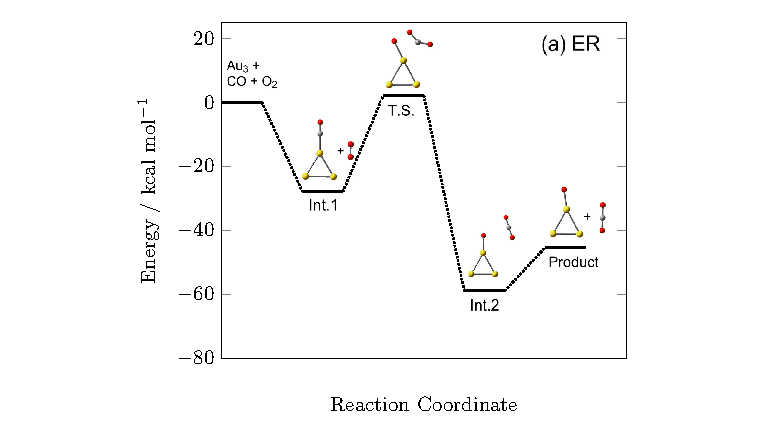
\includegraphics[width=0.455\textwidth,natwidth=610,
natheight=622,trim=2cm 0cm 2cm 0cm]
{Fig1a.pdf} }
              \fbox{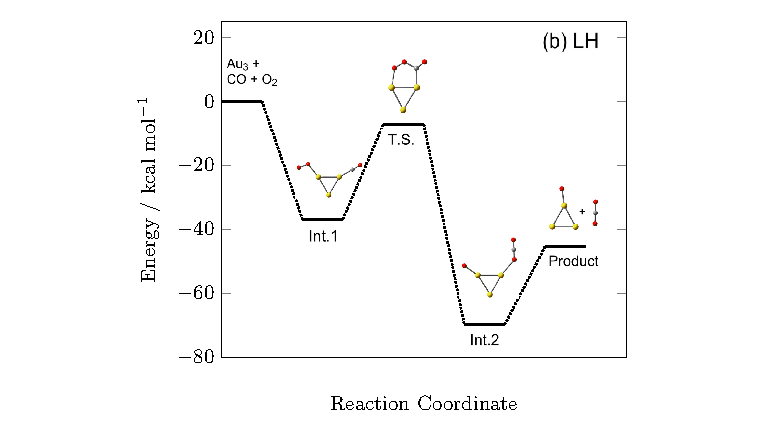
\includegraphics[width=0.455\textwidth, natwidth=610,natheight=622,trim=2cm 0cm 2cm 0cm]{Fig1b.pdf} } 
\caption{Complete representative reaction scheme for the Au$_3$ cluster catalyzed CO oxidation considering the (a) ER and (b) LH pathways.} \label{fig:rxn_mech}
\end{figure*}
As mentioned in the introduction, two mechanisms have been proposed for the CO oxidation reaction, ER and LH (Fig. \ref{fig:rxn_mech}). It is observed, in our study \cite{raipccp2015} and earlier works, that when following the ER mechanism, the reaction proceeds via a peroxo type transition state (T.S.) \cite{ping2010}. However, in case of the LH mechanism, the O--O bond length in the T.S. is similar to a superoxo type complex \cite{zhang2007,lopez2002,mavrikakis2003,liu2002,liu2003,ping2010}. 
Earlier reported results suggest that LH is the favored pathway in case of bare gold clusters being used as catalysts \cite{ping2010,Olga2010}. The preference for the LH pathway is attributed to the stability of the T.S. geometry obtained via the LH pathway over the one obtained via the ER pathway \cite{ping2010}. The preference of the LH pathway over ER, has also been explained on the basis of the fact of lower probability of head-on collisions between gas phase reactants (O$_2$) and surface bound reactants (CO) \cite{Jena2012,Olga2010,ping2010}.

\subsection{Adsorption of CO and coadsorption of CO and O$_{2}$ on the Au$_3$ cluster}
\begin{table}[!t]
\caption{The adsorption energy ($E_{\rm{adsorption}}$) is calculated with respect to the initial reactants, i.e., Au$_3$, CO and O$_2$. The barrier height ($E_{\rm{activation}}$) and energy of the reaction ($E_{\rm{reaction}}$) are calculated with respect to $E_{\rm{Int.1}}$ using different levels of theory. All values were calculated employing the SDD ECP and the 6-31+G* basis set, and are given in kcal/mol.} \label{error-bars}
\begin{small}
\begin{adjustbox}{max width=0.49\textwidth}
\begin{tabular}{|c|cc|cc|cc|}
\hline
 & \multicolumn{2}{c|}{$E_{\rm{adsorption}}$} & \multicolumn{2}{c|}{$E_{\rm{activation}}$} & \multicolumn{2}{c|}{$E_{\rm{reaction}}$}\\
\hline
Functional&$E_{\rm{Int.1}}^{\rm{ER}}$&$E_{\rm{Int.1}}^{\rm{LH}} $ &ER&LH&ER&LH\\
\hline
CCSD(T) &-27.91&-36.79&30.05&29.55&-31.08&-32.90\\
 B2PLYP-D&-30.18&-37.52&27.87&25.92&-37.06&-44.55\\
$\omega$B97xD&-30.80&-38.92&28.06&25.97&-38.44&-32.48\\
 cam-B3LYP&-30.49&-38.37&28.83&27.4&-37.97&-34.24\\
 lc-BLYP&-35.38&-47.60&25.41&23.17&-38.36&-32.84\\
  lc-$\omega$pbe&-33.84&-41.89&29.12&39.6&-37.07&-30.54\\
 O3LYP&-24.18&-29.30&28.55&26.55&-36.45&-26.61\\
X3LYP&-29.06&-37.48&24.8&25.58&-34.44&-29.48\\
HSE1PBE&-34.18&-42.83&25.09&24.26&-32.68&-28.69\\
MPW1K&-33.28&-40.88&26.53&24.9&-32.85&-29.18\\
B3PW91&-32.98&-41.11&25.62&24.94&-32.51&-27.26\\
B3P86&-35.16&-45.75&22.45&23.36&-32.88&-26.46\\
BHandLYP&-23.01&-24.96&33.03&14.28&-41.81&-41.59\\
PBE0&-34.49&-42.60&25.95&24.14&-31.01&-34.79\\
 BP86&-38.70&-54.82&13.66&22.49&-38.12&-23.33\\
PBE&-39.97&-56.39&12.81&21.78&-37.93&-23.72\\
BLYP&-31.05&-45.00&15.53&24.02&-40.39&-26.50\\
 M06L&-33.38&-49.01&13.78&22.84&-49.19&-37.30\\
TPSSh&-36.16&-49.87&18.45&24.84&-33.09&-23.33\\
VSXC&-30.08&-43.53&15.98&22.52&-43.46&-35.05\\
\hline
\end{tabular}
\end{adjustbox}
\end{small}
\begin{flushleft}
$E_{\rm{adsorption}}$ = $E_{\rm{Int.1}}$ - $E_{\rm{reactants}}$ ; $E_{\rm{activation}}$ = $E_{\rm{T.S.}}$ - $E_{\rm{Int.1}}$ ; $E_{\rm{reaction}}$ = $E_{\rm{Int.2}}$ - $E_{\rm{Int.1}}$
\end{flushleft}
\end{table}
Adsorption of the initial reactants on the surface of the catalyst is the first step in heterogeneous catalysis. In this respect, the adsorption energies were calculated using the nineteen different functionals mentioned in Table \ref{functionals}. The results are summarized in Table \ref{error-bars}, which indicates that coadsorption of CO and O$_2$ is favored over the adsorption of CO alone, irrespective of the level of theory employed. These results are in line with earlier reported experimental and theoretical works on the oxidation of CO using gold clusters as catalyst \cite{Olga2010,ping2010}. The adsorption of CO on Au$_3$ is an exothermic process and all the functionals overestimate the adsorption energy with respect to the CCSD(T) based results, except O3LYP and BHandHLYP, which underestimate the adsorption energy. Among the pure GGA functionals, VSXC and BLYP perform fairly well and overestimate the adsorption energy only by about 2 -- 3 kcal/mol, respectively. The inclusion of HF exchange component does not seem to systematically improve the result, though X3LYP shows good agreement with the CCSD(T) result. Addition of long range correlation to BLYP causes more deviation (7.5 kcal/mol) from the CCSD(T) result. This suggests that including the long range correction to the pure functional does not improve the description of the adsorption energetics of CO on Au$_3$. However, cam-B3LYP significantly improves the result, suggesting that together with the HF exchange component appropriately included, the long range corrected functionals are able of describe the adsorption energetics accurately. The inclusion of dispersion effects via the $\omega$B97xD functional is also close to the CCSD(T) based values. The dispersion corrected double hybrid functional, B2PLYP-D, shows a deviation of only 2.3 kcal/mol from the CCSD(T) result, thus, reproducing the adsorption energetics with fairly good accuracy. \\
The coadsorption of CO and O$_2$ is an important step when the reaction proceeds via the LH pathway. However, when the coadsorption of CO and O$_2$ is considered together, the performance of the functionals is not similar to that observed for CO adsorption. This may be because of the $\pi \rightarrow \pi^*$ and $n \rightarrow \pi^*$ interactions that take place when O$_2$ is present in the vicinity of CO. The performance of pure GGA functionals drops, owing to the incapability of accurately considering the $\pi \rightarrow \pi^*$ type charge transfer interactions. The hybrid functionals, X3LYP, etc., predict the energetics reasonably well which is further improved upon addition of long range correlation to the hybrid B3LYP. Inclusion of dispersion correction via the $\omega$B97xD functional also shows a significant improvement in the estimation of adsorption energetics for the reaction. We can thereby conclude that, X3LYP, cam-B3LYP and $\omega$B97xD are a good compromise between the accuracy and computational cost in order to study the (co)adsorption energetics of CO oxidation on gold cluster. The following sections present the performance of these functionals in accurately predicting the reactivity by examining the activation energies.

\subsection{Activation barriers along the ER and LH pathways}
In this section, the barrier heights obtained from the DFT functionals are compared to the results obtained from the CCSD(T) method. It has been previously shown that applying the conventional WFT based Hartree-Fock method overestimates the barrier heights in general \cite{zhao2004jpca}.However, addition of the correlation component by employing the CCSD(T) method tends to lower the barrier height. The core correlation and relativistic effects are tackled by the SDD basis set and ECP, which is known to give reliable results in this respect \cite{Assado2009}. Thus, we benchmark all the DFT functionals against the CCSD(T)/SDD$\cup$6-31+G* level of theory. The activation energies corresponding to the CO oxidation reaction along the ER and LH pathways are given in Table \ref{error-bars}. Comparison of the performance of the methods used here in predicting the energy barriers of CO oxidation in absence of the gold cluster is presented in Table S1 of the Supplementary Material. The barrier heights are calculated as the energy difference of the T.S. with respect to the corresponding Int.1 for the ER and LH mechanisms (Fig. \ref{fig:rxn_mech}). Since the energy barriers are computed as the energy differences between the transition states and the CO+O2/ CO adsorbed gold cluster, the basis set superposition errors (BSSE) are expected to cancel out. Recalculating the energy barriers by accounting for BSSE resulted in marginal change ($\leq$1 kcal/mol). The activation barriers are in the range of about 12 to 33 kcal/mol and 14 to 40 kcal/mol along the ER and LH mechanistic pathways, respectively, whereas the barrier heights are 30.1 and 29.6 kcal/mol at the CCSD(T) level. Such a wide range of the barriers given by different functionals further signifies the need for a systematic benchmark study. The deviations of the activation barriers with respect to those obtained at the CCSD(T) level are depicted in Fig. \ref{CCSDT-Diff}. A value of zero in the plots indicates a perfect agreement between the corresponding DFT method and the CCSD(T) method. While negative values in the plots indicate underestimation of the barriers, positive values indicate overestimation. \\
The pure GGA based functionals (BLYP, PBE, BP86) show high deviations from the CCSD(T). However, it is clear from Fig. \ref{CCSDT-Diff}, that the deviation in barrier height values from CCSD(T) results is higher for the ER pathway in general. This difference may be attributed to the nature of the T.S., which is peroxo in ER and superoxo in LH in terms of the O--O bonding. The inclusion of kinetic energy density in orbital definition (VSXC, TPSSh, M06-L) seems to improve the results systematically. However, the performance is comparable to the pure GGA based functionals, namely BP86, PBE and BLYP (Table \ref{error-bars}). Inclusion of HF component, systematically improves the prediction of barrier height (TPSSh). \\
The hybrid functionals (O3LYP, X3LYP, HSE1PBE, MPW1K, B3PW91, B3P86, BHandHLYP and PBE0) resulting from the use of Fock--Kohn--Sham operator, lead to a significant improvement in the estimation of barrier heights. BHandHLYP, however, overestimates the barrier height for ER and underestimates the same via the LH pathway and hence, it may be difficult to arrive at qualitative trends in similar systems. In all the other cases the barrier height is underestimated with respect to the CCSD(T) results. The deviation from the CCSD(T) results is similar for both ER and LH pathways, suggesting that the inclusion of HF exchange component improves the modeling of the bond breaking step. However, the percentage of HF component added to the DFT functional also seems to play a crucial role as in the case of BHandHLYP, where 50$\% $ of HF component rather produces inconsistent results. Hence, HF exchange component seems to play a crucial role in correctly predicting the barrier heights and reaction pathways. \\
Considering the fact that charge transfer interactions play an important role in describing the T.S. of CO oxidation \cite{Olga2010,ping2010}, the performance of some long-range corrected (LC) DFT functionals was tested. The long range correction when applied to pure DFT functional, BLYP, gives values close to the ones predicted by hybrid DFT methods (Table \ref{error-bars}). lc-$\omega$PBE overestimates the barrier height for LH pathway. However, when the long range correction is applied to the hybrid B3LYP (cam-B3LYP), the results systematically improve and the barrier height is close to the CCSD(T) result. It can thus be concluded from here that charge transfer interactions in both T.S. and intermediates need to be properly treated for the correct prediction of the barrier height. \\
\begin{figure}[!t] 
            \centering
               \fbox{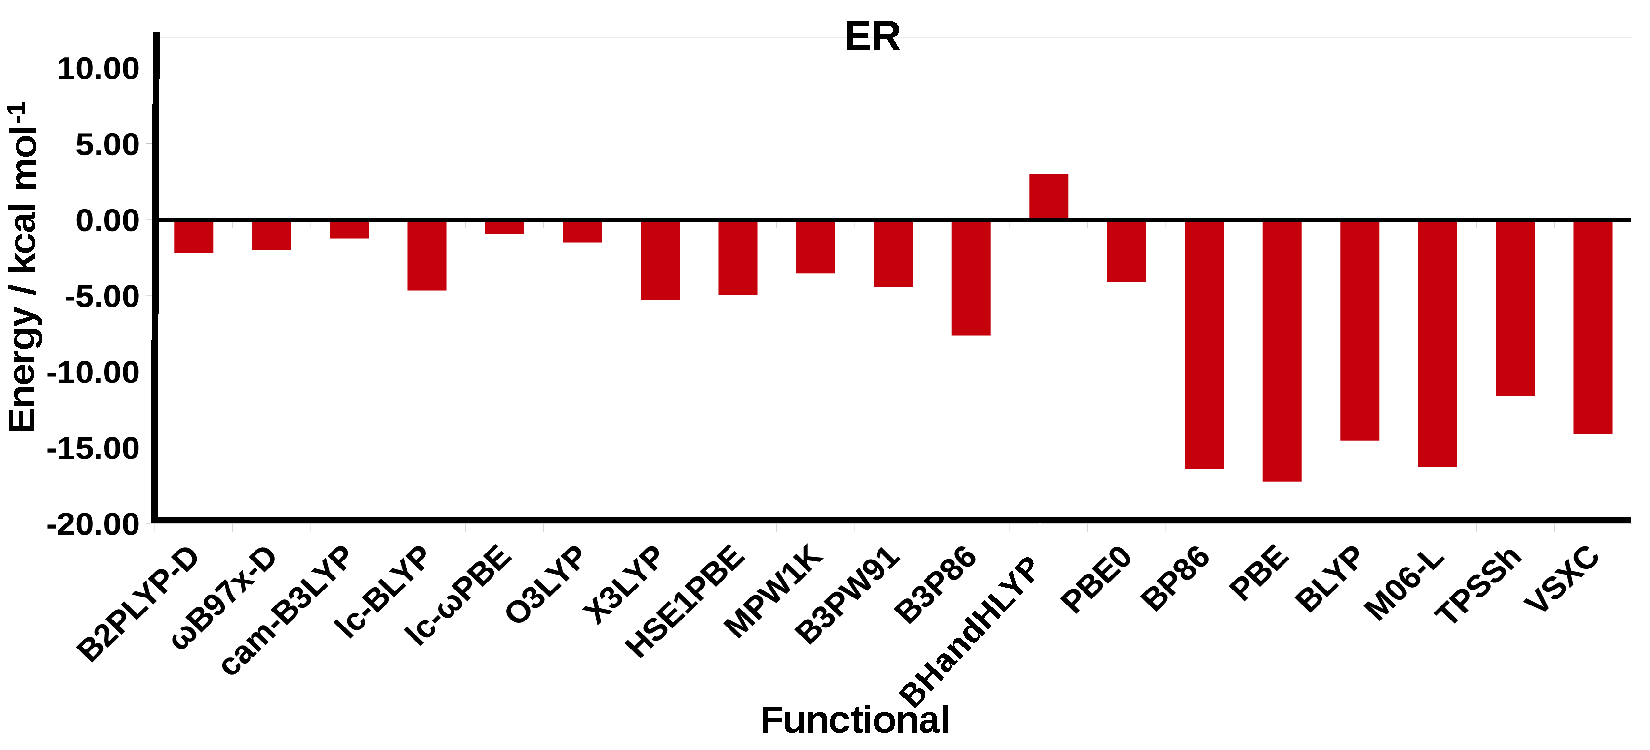
\includegraphics[width=0.48\textwidth, natwidth=610,natheight=642]{Fig2a.pdf} }
              \fbox{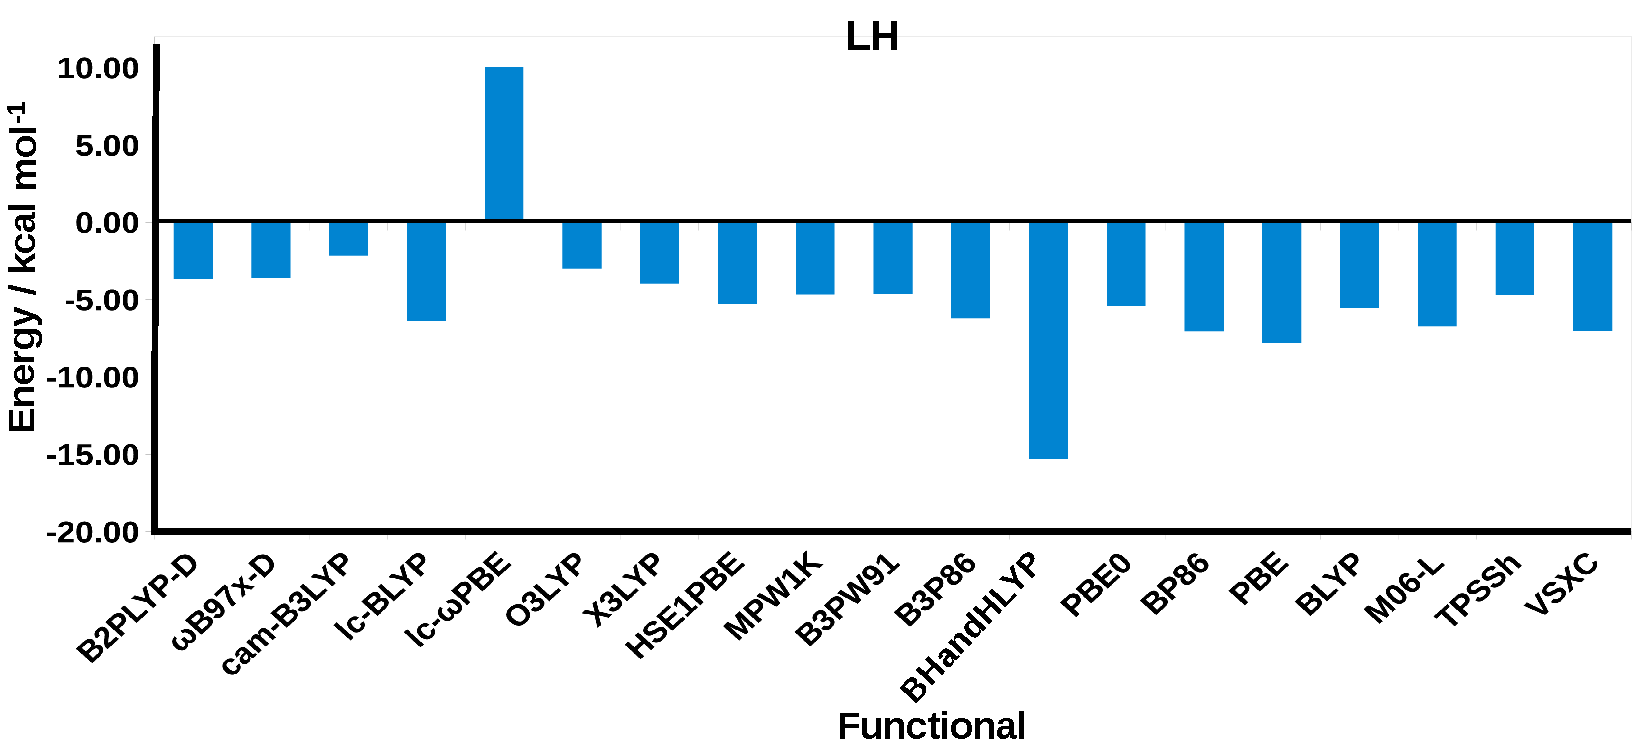
\includegraphics[width=0.485\textwidth, natwidth=610,natheight=642]{Fig2b.pdf}}
\caption{Deviation in the energy values of the T.S. with respect to CCSD(T) level of theory. The mean negative deviation corresponding to ER is 8.5 kcal/mol and for LH it is 6.1 kcal/mol. Negative value indicates that the functional underestimates the barrier height, whereas a positive value indicates overestimation. All values were calculated employing the SDD ECP and the 6-31+G* basis set, and are given in kcal/mol.} \label{CCSDT-Diff}
\end{figure}
Hybrid GGA functionals are further systematically improved by addition of dispersion correction term that is a relatively simple function of interatomic distances and contains adjustable parameters that are fitted to conformational and interaction energies computed using CCSD(T)/CBS \cite{grimme2006,grimme2007,grimme2011}. The addition of dispersion correction was tested for an LC corrected functional, $\omega$B97x-D. The results hardly improve upon inclusion of dispersion correction suggesting that in this case, dispersion does not seem to play a significant role in on the energetics of the T.S. A previous study has suggested that the use of a double hybrid functional results in good estimation of barrier height when studying reaction pathways \cite{svelle2009}. Though the double hybrid functional (B2PLYP-D), which includes a certain amount of HF exchange and PT2 correlation \cite{grimme2006,grimme2007}, provides a good agreement, the computational cost of these calculations is similar to MP2 level calculations. Based on these calculations, it can be suggested that $\omega$B97x-D and cam-B3LYP give a good estimation of barrier height. However, the global hybrid functionals, O3LYP, X3LYP, HSE1PBE, PBE0, MPW1K and B3PW91, perform consistently irrespective of the pathway followed, with a deviation within $\sim$ 5 kcal/mol. Barrier heights were calculated using the 6-311+G* basis set at the PBE0 level of theory, and it was observed that the values increased by about 0.5 kcal/mol in case of ER pathway, and 1.0 kcal/mol in case of LH pathway.

\subsection{Preference of the LH vs ER pathway for the CO oxidation}
\begin{figure}[!t]
\centering
\fbox{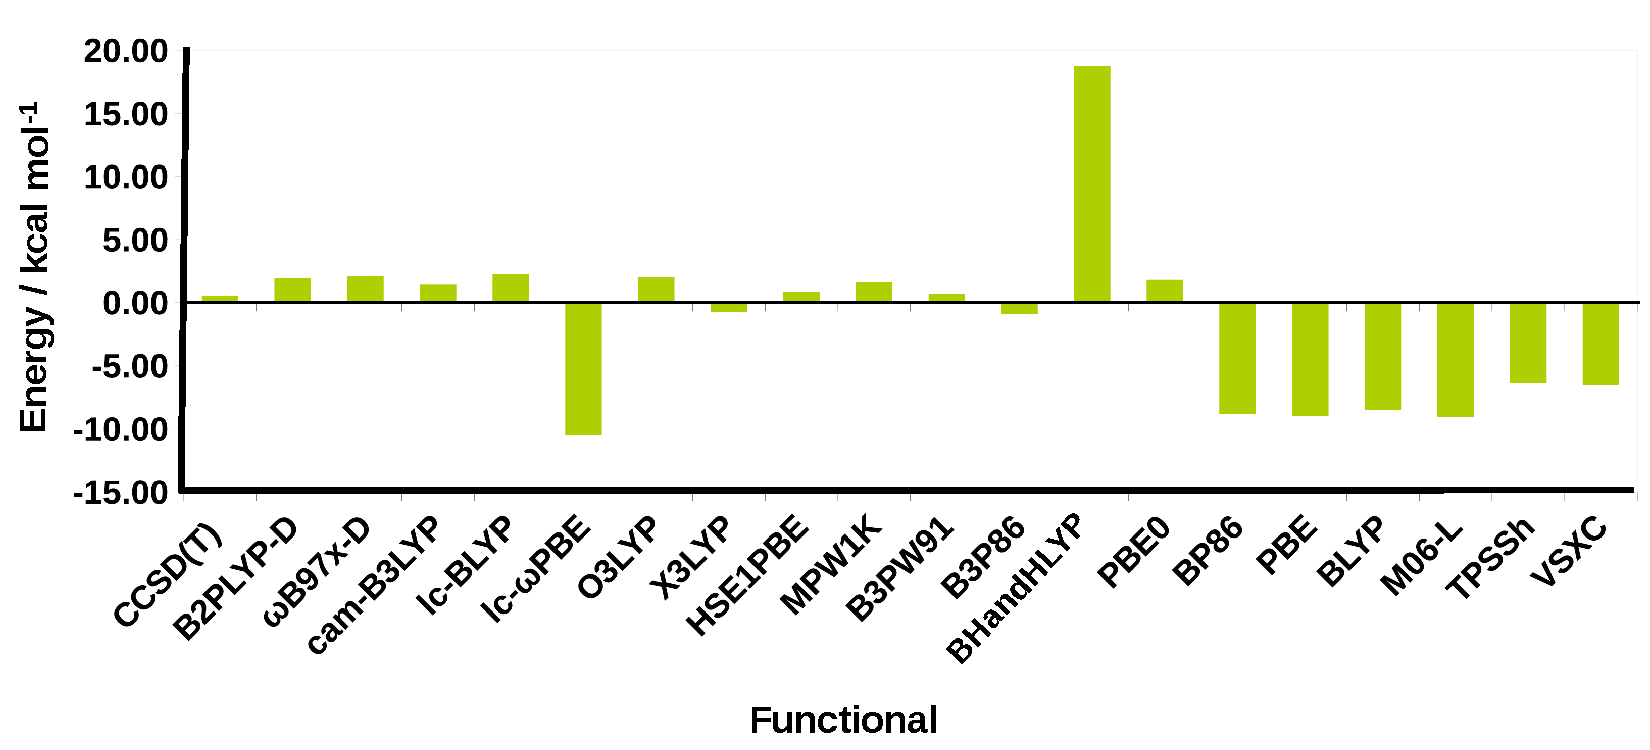
\includegraphics[width=0.485\textwidth, natwidth=610,natheight=642]{Fig3.pdf}}
\caption{Difference between the $E_{\rm{activation}}^{\rm{ER}}$--$E_{\rm{activation}}^{\rm{LH}}$ corresponding to all the functionals along with the difference calculated at CCSD(T) level in kcal/mol. Positive values indicate a preference for LH pathway over ER and negative values suggest that ER pathway is preferred over the LH pathway. All values were calculated employing the SDD ECP and the 6-31+G* basis set, and are given in kcal/mol.} \label{ER-LH-diff}
\end{figure}
Previous computational and experimental studies have shown that the LH mechanistic pathway is more preferred over the ER pathway \cite{Jena2012,Olga2010,ping2010}. The ability of the different functionals used to predict the correct preference for the reaction pathways and the energy difference between the two barrier heights is discussed here. The results have been summarized in Fig. \ref{ER-LH-diff}, where a positive value indicates a preference for LH pathway over the ER pathway, whereas, a negative value suggests the opposite. \\
According to the CCSD(T) calculations, the LH pathway is favored by an energy difference of 0.5 kcal/mol, whereas the numbers lie in the range of 18 to -15 kcal/mol for the DFT methods. Several functionals predict ER to be more favored energetically, not in consensus with the existing data. All the pure GGA functionals (BLYP, PBE and BP86) and the meta GGA functionals, both pure (VSXC and M06-L) and hybrid (TPSSh), predict the ER pathway to be more favorable for the CO oxidation on gold cluster. On inclusion of the HF exchange component, all the resulting hybrid functionals correctly predict the preference for LH mechanism over ER, with the only exception of B3P86 and X3LYP, which suggests ER to be more favorable by $\sim$0.78 kcal/mol. This hints towards the importance of the HF exchange component in correctly predicting the reaction pathways. However, the inclusion of long range correction to the pure GGA PBE functional (lc-$\omega$PBE) is unable to predict the preference for the LH pathway over the ER pathway. The deviation occurring in case of lc-$\omega$PBE can be attributed to its pure GGA character, emphasizing the importance of the inclusion of the HF exchange component. Apart from these anomalies, all the hybrid functionals with long range and/or dispersion corrections incorporated, are able to correctly predict the preference for LH pathway over the ER pathway. However, it is to be noted that the quantity $E_{\rm{activation}}^{\rm{ER}}$--$E_{\rm{activation}}^{\rm{LH}}$ shows a deviation from the CCSD(T) predicted values and in all the cases this difference is overestimated. Hence, in terms of a quantitative estimation, the hybrid DFT functionals, B3PW91 and HSE1PBE are able to reproduce the difference more closely to the CCSD(T) level estimated value (Fig. \ref{ER-LH-diff}), though the reaction barriers are underestimated by 5 kcal/mol. These results suggest that the hybrid DFT functionals perform fairly good in terms of giving a qualitatively accurate picture of the mechanistic pathway for CO oxidation on a gold cluster.

\subsection{Energetics of the reaction}
\begin{figure}[!t]
        \centering
               \fbox{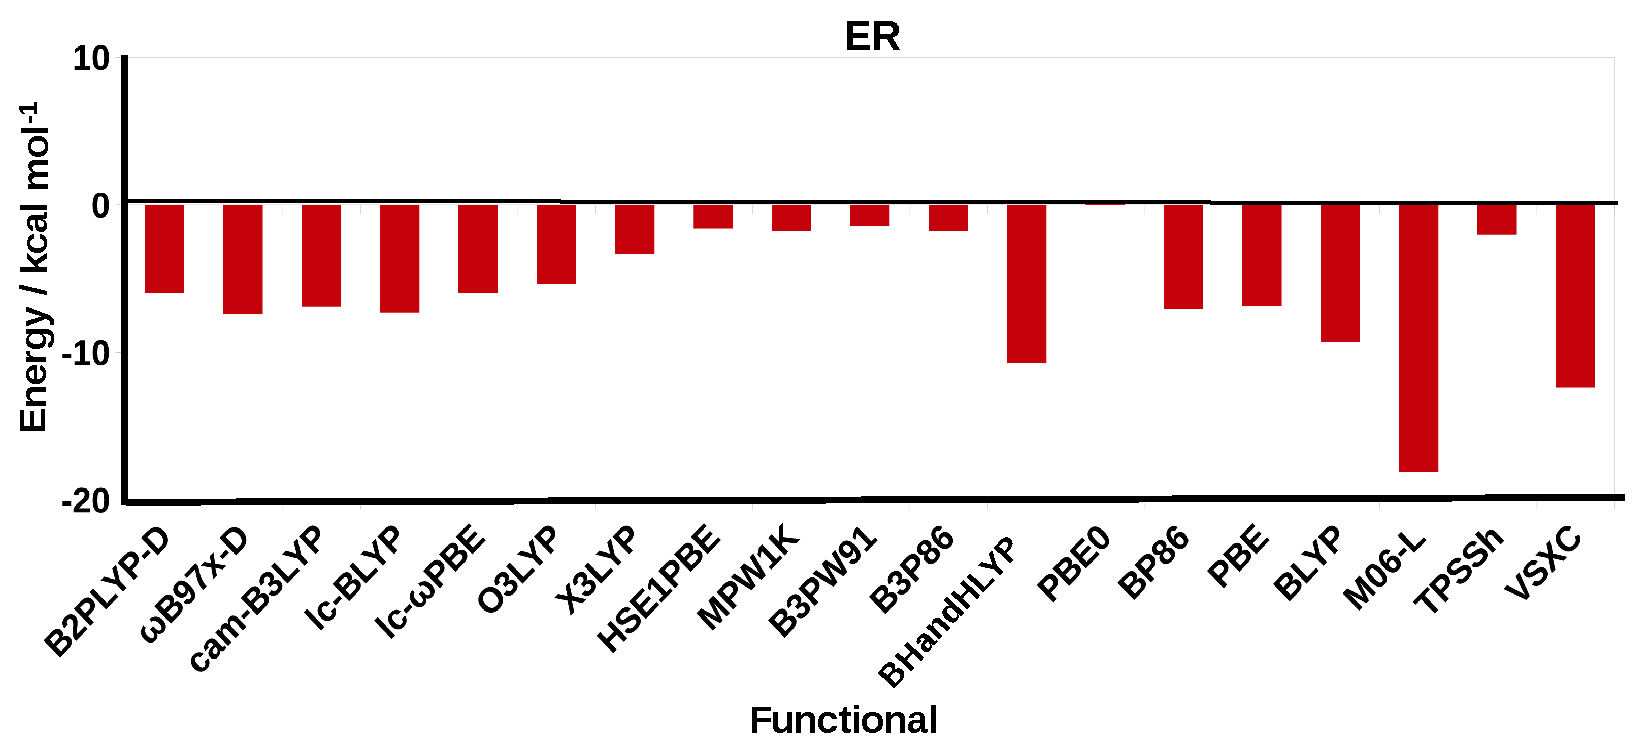
\includegraphics[width=0.48\textwidth, natwidth=610,natheight=642]{Fig4a.pdf} }
              \fbox{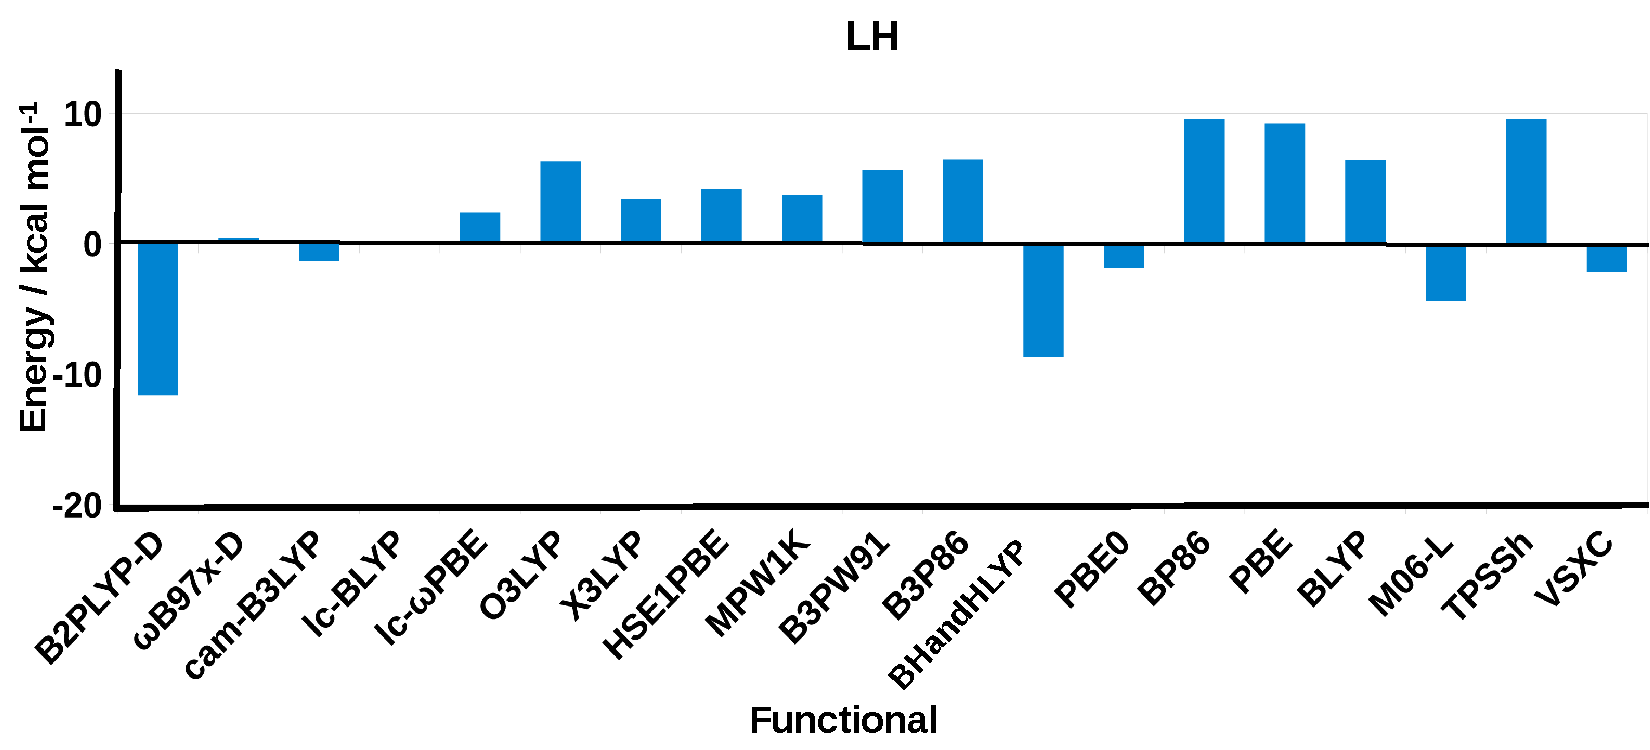
\includegraphics[width=0.485\textwidth, natwidth=610,natheight=642]{Fig4b.pdf}}
\caption{Deviation in the reaction energy ($E_{\rm{reaction}}$) value with respect to CCSD(T) level of theory. Negative values indicate that the functional overestimates the reaction energy, whereas a positive values indicate an underestimation of the same. All values were calculated employing the SDD ECP and the 6-31+G* basis set, and are given in kcal/mol. } \label{energetics_diff_ccsd}
\end{figure}
Reaction energy is an important parameter in order to understand the complete reaction profile. In this section, the reaction energies obtained using different DFT functionals are compared to the CCSD(T) results. The reaction energy is calculated as the energy difference between the corresponding Int.1 and Int.2 for both ER and LH pathways (Fig. \ref{fig:rxn_mech}), as these are the steps where the gold cluster plays role in stabilizing the intermediates. The reaction energies span a wide range of values from -31.0 to -49.2 kcal/mol corresponding to the ER mechanism and -18.9 to -44.5 kcal/mol corresponding to the LH mechanism. The values obtained using the CCSD(T) method are -31.1 and -32.9 kcal/mol for the ER and LH mechanisms, respectively. Notably, the reaction energy corresponding to the CO oxidation reaction in absence of the catalyst calculated at the same level is -7.1 kcal/mol. Such a large difference between the two reactions is due to the fact that an atomic oxygen is adsorbed on the gold cluster in the product in presence of the catalyst. Fig. \ref{energetics_diff_ccsd} summarizes the deviation of all the DFT functionals with respect to the CCSD(T) level results, which shows a clear difference in the estimation of the reaction energies corresponding to the ER and LH mechanisms. \\
For the ER mechanism, the stabilization energy of the reaction is overestimated using all the DFT functionals, with respect to the CCSD(T) level value. The deviation is large for meta-GGA functionals. This suggests that these functionals tend to overstabilize the product of the reaction compared to the CCSD(T) level. The hybrid GGA functionals significantly improve the reaction energy values. Except BHandHLYP, all other hybrid functionals predict the reaction energy within $\sim$ 6 kcal/mol deviation from the CCSD(T) value. This suggests that inclusion of HF exchange term is responsible for achieving the correct energetic picture of the present reaction. Further improvement of the functionals by addition of long range correction and dispersion correction does not seem to play a significant role in predicting the correct energetics of the reaction. PBE0 shows an excellent agreement with the CCSD(T) predicted values.\\  
The reaction energy trends via the LH pathway are different from the ER pathway, as certain functionals underestimate the reaction energy values. This disagreement of either overestimation or underestimation of reaction energy with respect to a standard value may lead to a qualitatively wrong picture of the reaction energetics. Hence, the functionals which inconsistently overestimate/underestimate the values corresponding to  two pathways, cannot be used to yield reliable results for this reaction. Among the hybrid functionals, only PBE0 and BHandHLYP perform consistently. The long range corrected lc-BLYP and cam-B3LYP and the dispersion corrected B2PLYP-D also perform consistently, irrespective of the pathway followed. Of all the functionals used, PBE0 results lie in close agreement with the CCSD(T) values for both ER and LH mechanisms.
\subsection{Comparison of the geometries obtained using different DFT functionals}
\begin{figure}[!t]
\begin{center}
        \centering
               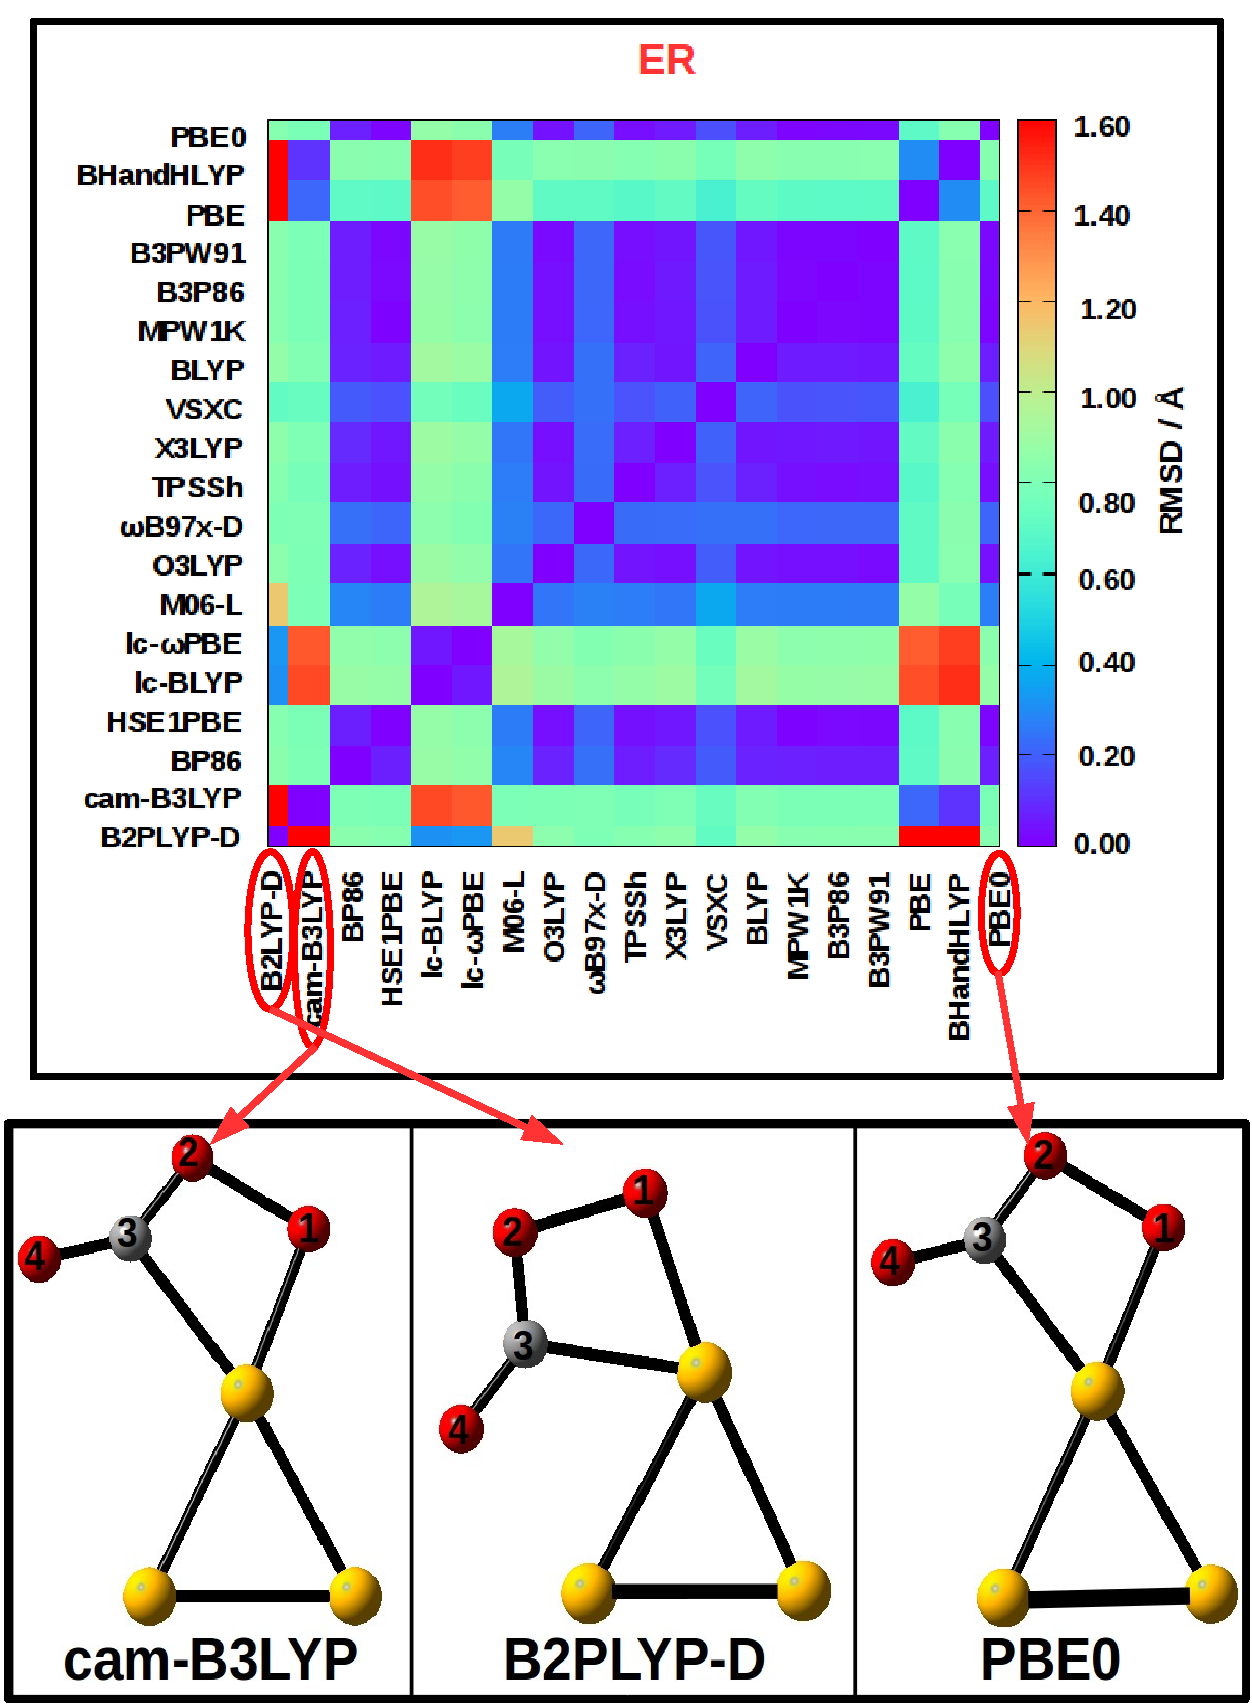
\includegraphics[width=0.4195\textwidth, natwidth=610,natheight=642]{Fig5a.pdf} 
               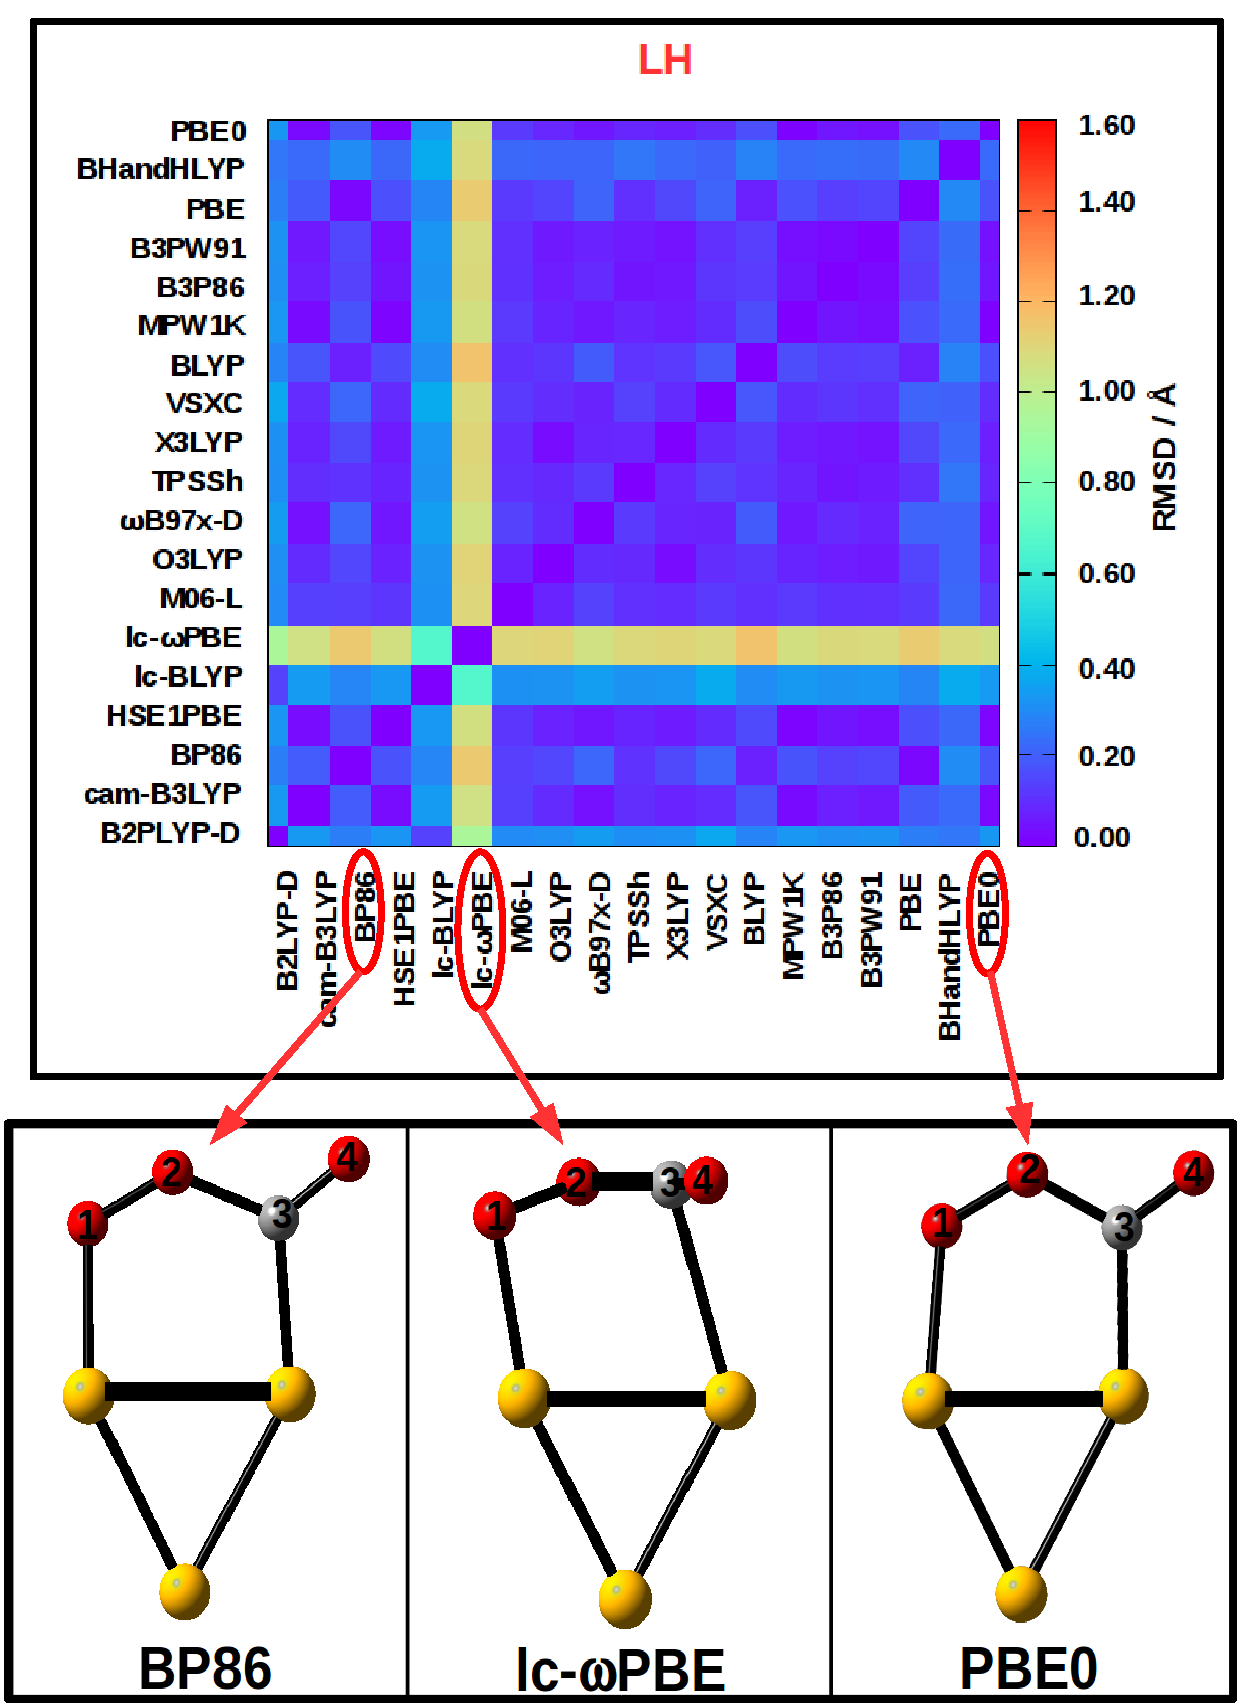
\includegraphics[width=0.4195\textwidth, natwidth=610,natheight=642]{Fig5b.pdf} 
\caption{Root mean square deviation (RMSD / \r{A}) with respect to all the functionals for T.S. via both ER and LH mechanisms. Shown below are the optimized geometries of the transition states obtained using the PBE0 level, and use the functional pairs that exhibit the maximum RMSD value.}     \label{fig:TS}          	              
\end{center}
\end{figure}
\begin{table}[!ht]
\caption{Bond length of O$_2$ ($r_{\rm{O-O}}$ in \r{A}) and the charge gained/lost by the gold cluster ($\Delta q$) during the formation of Int1 ($\Delta q_{\rm{Int.1}}$) and at the saddle point ($\Delta q_{\rm{T.S.}}$). All values were calculated employing the SDD ECP and the 6-31+G* basis set.} \label{geom:error-bars}
\begin{small}
\begin{adjustbox}{max width=0.493\textwidth}
\begin{tabular}{|c|cc|cc|cc|}
\hline
&\multicolumn{2}{c|}{r$_{O-O}$}&\multicolumn{2}{c|}{$\Delta q_{Int.1}$}&\multicolumn{2}{c|}{$\Delta q_{T.S.}$}\\
\hline
Functional&ER&LH&ER&LH&ER&LH\\
\hline
 B2PLYP-D&1.66&1.39&0.228&0.509&0.333&0.542\\
$\omega$B97x-D&1.70&1.36&0.219&0.437&0.300&0.400\\
 cam-B3LYP&1.70&1.37&0.194&0.434&0.301&0.394\\
 lc-BLYP&1.64&1.42&0.160&0.482&0.217&0.435\\
  lc-$\omega$PBE&1.65&1.48&0.251&0.531&0.229&0.339\\
 O3LYP&1.73&1.36&0.428&0.533&0.354&0.480\\
X3LYP&1.72&1.37&0.234&0.392&0.272&0.393\\
HSE1PBE&1.72&1.36&0.283&0.400&0.284&0.937\\
MPW1K&1.72&1.36&0.316&0.454&0.307&0.414\\
B3PW91&1.73&1.36&0.281&0.406&0.283&0.385\\
B3P86&1.73&1.36&0.240&0.366&0.269&0.368\\
BHandHLYP&1.67&1.30&0.226&0.469&0.313&0.472\\
PBE0&1.72&1.35&0.298&0.423&0.295&0.406\\
 BP86&1.78&1.37&0.258&0.329&0.243&0.330\\
PBE&1.78&1.36&0.327&0.396&0.275&0.373\\
BLYP&1.77&1.39&0.246&0.362&0.252&0.355\\
 M06-L&1.40&1.35&0.167&0.285&0.308&0.366\\
TPSSh&1.75&1.38&0.350&0.465&0.316&0.400\\
VSXC&1.71&1.37&0.334&0.402&0.276&0.378\\
\hline
\end{tabular}
\end{adjustbox}
\end{small}
\end{table}  
The geometries of each of the stationary points obtained using the different DFT
functionals are compared with each other. Initially, the comparison of the overall structures is made by calculating the root mean square deviations (RMSD). Structures of Int.1 along the ER pathway obtained using all the nineteen functionals are taken, and every possible pair is superimposed on each other considering only the three gold atoms. Based on the superimposed structures, the RMSD for the whole structure is calculated. This is repeated for T.S., and Int.2, along the ER and LH pathways. The RMSD data corresponding to the Int.1 and Int.2 are given in the Supplementary Material as heat maps. The data, which show a maximum deviation of 0.5 \r{A}, reveal general consistency of the functionals used here in predicting the geometry of the minimum energy structures. A similar analysis is done on the T.S. along the two pathways and the results are depicted in Fig. \ref{fig:TS}. Additionally, the O--O distances in the T.S. structures are given in Table \ref{geom:error-bars}. All the functionals predict the formation of a superoxo complex for T.S. corresponding to LH mechanism and a peroxo complex for the ER mechanism (with an exception of M06-L, that predicts a superoxo complex in both cases). However, unlike the structures of Int.1 and Int.2, larger deviations are observed with some of the functionals, which is traced mainly due to the changes in the planarity in the structure. For the ER pathway, B2PLYP-D, cam-B3LYP, lc-BLYP and lc-$\omega$PBE show a large deviation with respect to all other functionals.  In case of the LH mechanism, lc-$\omega$PBE shows high RMSD value with respect to all the other functionals used (Fig. \ref{fig:TS}). Most of the functionals agree with each other with an RMSD difference of less than 0.5 \r{A} as in the case of Int.1 and Int.2. For example, in case of LH, comparison of the structures obtained using all functionals, except lc-$\omega$PBE, exhibits low RMSD values (Fig. \ref{fig:TS}). In lc-$\omega$PBE, the C3-O4 does not remain in plane of the cluster, thus explaining the high deviation. However, for ER the functionals B2PLYP-D, cam-B3LYP, lc-BLYP and lc-$\omega$PBE lead to geometries where the O4 atom forms an interaction with the neighboring Au atom, thus causing a bend of the total O1-O2-C3-O4 complex leading to higher RMSD values (Fig. \ref{fig:TS}). \\
It is noted that the optimization of one of the final products, atomic oxygen adsorbed on Au$_3$, results in two different local minima, one where O atom interacts with one Au atom of the cluster and the other, where oxygen atom interacts with two Au atoms simultaneously, depending on the DFT functional used (Figure S2 of the Supplementary Material). A set of functionals i.e. cam-B3LYP, lc-BLYP, BLYP and BHandHLYP predict structure B as minimum, whereas, all the other functionals predict structure A to be the minimum energy structure. Hence, in this case we find a difference in the prediction of correct geometry using different DFT functionals. On comparing the CCSD(T) energy values for both A and B, we find A to be stable by 2.1 kcal/mol and thus can be considered to be the actual minimum energy geometry.

\subsection{Charge transfer analysis for Int.1 and T.S.}
Mulliken charge analysis was done on T.S. for all the nineteen functionals (Table \ref{geom:error-bars}). The charge gained or lost by Au$_3$ on the formation of Int.1 or T.S. complex is defined by the quantity, $\Delta q$. The charge analysis for Int.1 and T.S. was done for both the pathways. Corresponding to Int.1, it is observed that a charge transfer from the cluster to the adsorbed reactants takes place, irrespective of any functional used. However, the amount of charge transfer is higher for the LH pathway. Similarly, in the T.S., we find charge being transferred from the cluster catalyst to O--O in all cases. This is important for the activation of the O--O bond and thus, the oxidation of CO. Again, we find that a similar qualitative picture is given by even the pure DFT functionals. It can thus be conjectured here that DFT functionals also give a good qualitative picture in terms of the direction of charge transfer occurring, which in this case is from the gold cluster to the $\pi^*$ orbital of O$_2$.

\section{Summary}
This paper reports benchmark calculations for the adsorption energy, barrier height, reaction energy and T.S. geometry of the oxidation of CO via O$_2$ using gold cluster (Au$_3$) as the catalyst via the ER and LH mechanisms. Calculations performed at the CCSD(T) level predict the codasorption of CO and O$_2$ on the gold cluster to be more favorable in comparison to the adsorption of CO alone. This picture is correctly reproduced by all the functionals considered in this work. However, inclusion of long range and dispersion corrections (cam-B3LYP, $\omega$B97x-D) seem to improve the quantitative accuracy of the calculations, indicating the role of long range and dispersion interactions in the adsorption process. CCSD(T) calculations and earlier reported results indicate a preference for LH pathway. The reaction is predicted to be exothermic irrespective of the pathway followed. In terms of E$_{\rm{activation}}$, B2PLYP-D, $\omega$B97x-D, cam-B3LYP, O3LYP, X3LYP, HSE1PBE, MPW1K, B3PW91 and PBE0 are able to predict the value with fairly reasonable accuracy within 6 kcal/mol. We emphasize on the fact that inclusion of HF exchange is important for correctly predicting the favorable pathway, but that needs to be done cautiously. Incorporation of long range correction improves the prediction of barrier height; however, dispersion corrections do not seem to play much role. The reaction energy is overestimated by all the functionals in case of ER pathway, but corresponding to LH mechanism the same is underestimated in some cases. Compared to all other functionals, PBE0 and cam-B3LYP show better agreement with CCSD(T) results. While the ground state geometry for Au$_3$-O is correctly predicted by PBE0, the one predicted by cam-B3LYP is 2.1 kcal/mol higher, as per the CCSD(T) results. Thus, on the basis of the benchmark results, we identify the hybrid DFT functionals, PBE0, B3PW91 and B3P86, as reasonable choices in terms of predicting the barrier height and thermochemical data within an affordable computational range even if the system size grows larger. This benchmark study is done using the SDD ECP and 6-31+G* basis set. However, calculations using the triple-$\zeta$ 6-311+G* basis set at the PBE0 level yielded similar results. Since this benchmark study is done on a specific reaction, i.e., oxidation of CO, caution must be exercised while extending the conclusions arrived here on other systems. Such studies on other reactions are expected to provide a generalized trend on the performance of the DFT functionals in modeling reactions catalyzed by metal clusters and nanoparticles.

\begin{acknowledgements}
S. R. acknowledges support from CSIR for SRF fellowship. M.E. acknowledges the financial support from a Grant-in-Aid for Scientific Research from the Japan Society for the Promotion of Science (JSPS), Nanotechnology Platform Program of the Ministry of Education, Culture, Sports, Science, and Technology (MEXT) of Japan.
\end{acknowledgements}

% BibTeX users please use
\bibliographystyle{spbasic1}
%\bibliographystyle{springer}
\bibliography{Benchmarking}   % name your BibTeX data base

% Non-BibTeX users please use
%\begin{thebibliography}{3}
%
% and use \bibitem to create references. Consult the Instructions
% for authors for reference list style.
%
% Format for Journal Reference

\end{document}
% end of file template.tex
